% ============================================================
%  SE(2)-Equivariant RoadNet -- Vietnamese presentation slides
%  Method: exp02_SE2Equivariant.py  (with RoadFury baseline from exp00)
%  Audience: thesis advisor (thay) -- RoadFury -> SE2 narrative
%  Compile: pdflatex se2_slides.tex (twice for TOC/refs)
%  Engine: pdfLaTeX with TeX Live (vietnam.sty + utf8)
% ============================================================
\documentclass[aspectratio=169,10pt]{beamer}

\usetheme{metropolis}
\usecolortheme{metropolis}
\usefonttheme{professionalfonts}
\setbeamertemplate{frame numbering}[fraction]
\setbeamertemplate{itemize item}{\textcolor{mLightBrown}{\scriptsize$\blacktriangleright$}}
\setbeamertemplate{itemize subitem}{\textbullet}
\setbeamertemplate{itemize subsubitem}{--}

% -- Packages --
\usepackage{amsmath, amssymb}
\usepackage[utf8]{inputenc}
\usepackage{vietnam}
\usepackage[english]{babel}
\usepackage{booktabs}
\usepackage[table]{xcolor}
\usepackage{tikz}
\usepackage{pgfplots}
\usepackage{array}
\usepackage{graphicx}
\usepackage{adjustbox}
\usepackage{hyperref}
\pgfplotsset{compat=1.18}
\usetikzlibrary{shapes.geometric, arrows.meta, positioning, calc, fit, backgrounds, decorations.pathmorphing}

% ============================================================
%  PALETTE  (matches summary_proposal.tex)
% ============================================================
\definecolor{mDarkTeal}{HTML}{23373B}
\definecolor{mLightBrown}{HTML}{EB811B}
\definecolor{softgray}{HTML}{F2F4F7}
\definecolor{tealtint}{HTML}{D6DEE0}

\colorlet{navydeep}{mDarkTeal}
\colorlet{navymid}{mDarkTeal!75}
\colorlet{accent}{mLightBrown}
\colorlet{success}{green!50!black}
\colorlet{alert}{red!70!black}
\colorlet{lightnavy}{tealtint}

\hypersetup{colorlinks=true, urlcolor=mLightBrown, linkcolor=mDarkTeal}
\renewcommand{\arraystretch}{1.15}

% Path helpers
\graphicspath{{./figures/}{./slide/figures/}{../figures/}{../paper/}{../paper/present/}{../slides/latex_proposal/}}

% Safe-include: hien thi placeholder neu file chua co.
% Dung: \safeincludegraphics[width=...]{tenfile.png}{Caption neu missing}
\newcommand{\safeincludegraphics}[3][width=\linewidth]{%
  \IfFileExists{#2}{\includegraphics[#1]{#2}}{%
    \IfFileExists{./figures/#2}{\includegraphics[#1]{./figures/#2}}{%
      \IfFileExists{../paper/#2}{\includegraphics[#1]{../paper/#2}}{%
        \IfFileExists{../paper/present/#2}{\includegraphics[#1]{../paper/present/#2}}{%
          \IfFileExists{../slides/latex_proposal/#2}{\includegraphics[#1]{../slides/latex_proposal/#2}}{%
            \fbox{\parbox[c][3.6cm][c]{0.85\linewidth}{\centering\scriptsize
              \textbf{[placeholder image]}\par\vspace{2pt}
              \texttt{\detokenize{#2}}\par\vspace{4pt}
              \itshape #3}}%
          }%
        }%
      }%
    }%
  }%
}

% ---- TikZ styles for pipeline block diagrams (shared) ----
\tikzset{
  pipefont/.style={font=\sffamily\scriptsize},
  blk/.style={draw, rounded corners=2pt, fill=#1, align=center,
              inner sep=3pt, minimum width=2.7cm, minimum height=0.74cm,
              font=\sffamily\scriptsize},
  grp/.style={draw=#1!60, dashed, rounded corners=5pt,
              inner sep=6pt, fill=#1!7},
  htitle/.style={font=\sffamily\bfseries\footnotesize},
  parr/.style={->, thick, >=Stealth},
}

% ============================================================
%  TITLE METADATA
% ============================================================
\title{Test Prioritization for Self-Driving Cars -- ICST 2026}
\author{Trần Chí Nguyên, Huỳnh Trung Kiệt, Đào Sỹ Duy Minh}
\institute{University of Science, VNU-HCM}
\date{ICST 2026}

\begin{document}

% ============================================================
% 1. TITLE
% ============================================================
{
\setbeamertemplate{footline}{}
\begin{frame}
\vspace{0.4em}
\begin{columns}[c]
\column{0.18\textwidth}
\centering

\includegraphics[height=2.0cm]{hcmus.png}

\column{0.64\textwidth}
\centering
\large\textbf{The Self-Driving Car Testing Competition}\\[0.3em]
\footnotesize organized jointly by the International Conference on\\
Software Testing, Verification and Validation \textbf{(ICST)}\\[0.7em]
\large\textcolor{navydeep}{\textbf{Test Prioritization for Self-Driving Cars}}\\[0.2em]
\normalsize\textbf{ICST 2026}

\column{0.18\textwidth}
\centering

\includegraphics[height=1.6cm]{icst_logo.jpg}
\end{columns}

\vspace{1.8em}
\begin{columns}[c]
\column{0.18\textwidth}
\column{0.64\textwidth}
\begin{block}{Team Members}
\scriptsize
\begin{itemize}
  \item Trần Chí Nguyên -- 23102244
  \item Huỳnh Trung Kiệt -- 23122039
  \item Đào Sỹ Duy Minh -- 23122041
\end{itemize}
\end{block}
\column{0.18\textwidth}
\end{columns}

\vspace{1.2em}
\centering
\scriptsize University of Science, VNU-HCM
\end{frame}
}

% ============================================================
% 2. AGENDA
% ============================================================
\begin{frame}{Nội dung trình bày}
\begin{enumerate}
    \item \textbf{Overview Problem}
    \item \textbf{Input, Output \& Dataset}
    \item \textbf{Methodology}
    \item \textbf{Evaluation}
    \item \textbf{Leaderboard}
    \item \textbf{Conclusion}
\end{enumerate}
\end{frame}

% ============================================================
% PART I -- OVERVIEW
% ============================================================
\section{Overview Problem}

% --- Hero / Big picture ---
\begin{frame}{Bối cảnh: SDC Testing Competition}
\begin{columns}[T]
\column{0.55\textwidth}
\begin{block}{Vì sao cần kiểm thử SDC trong mô phỏng?}
\scriptsize
\textbf{Self-driving cars} là hệ thống phần mềm-vật lý phức tạp: một thay đổi nhỏ có thể làm xe lệch làn ở kịch bản hiếm.
\begin{itemize}
    \item Kiểm thử ngoài đời thật đắt, chậm và khó.
    \item Mô phỏng cho phép chạy hàng ngàn road scenarios.
    \item Nhưng chạy trên toàn bộ test vẫn rất tốn kém.
\end{itemize}
\end{block}

\begin{exampleblock}{Bài toán của competition}
\scriptsize
Với một tập test Self-driving Cars lớn, mục tiêu là: chọn và xếp thứ tự các kịch bản sao cho lỗi được phát hiện càng sớm càng tốt.
\end{exampleblock}

\column{0.42\textwidth}
\centering
\safeincludegraphics[width=\linewidth, keepaspectratio]{fig_hero_sdc.png}{Gemini: xe tu lai tren duong cong}\\[0.3em]
\scriptsize\textit{Trong mỗi kịch bản, xe phải giữ làn trên một đường cụ thể; FAIL xảy ra khi xe lệch khỏi làn.}
\end{columns}
\end{frame}

% --- Why prioritize ---
\begin{frame}{Vì sao cần ưu tiên kiểm thử?}
\begin{columns}[T]
\column{0.48\textwidth}
\centering
\safeincludegraphics[width=\linewidth, keepaspectratio]{fig_problem_motivation.png}{Gemini: motivation -- ngan test, can rank}\\[0.3em]
\scriptsize\textit{Ngàn kịch bản $\to$ chỉ cần chạy ít kịch bản đầu là đủ thấy lỗi.}

\column{0.50\textwidth}
\begin{block}{Bài toán ưu tiên kiểm thử (Test Prioritization)}
\small
\begin{itemize}
    \item Nếu xếp hạng tốt $\Rightarrow$ phát hiện lỗi sớm $\Rightarrow$ \textbf{cắt 50--80\%} thời gian testing.
    \item Nếu xếp hạng kém $\Rightarrow$ lỗi nằm ở cuối hàng đợi $\Rightarrow$ tốn nhiều chi phí và thời gian.
\end{itemize}
\end{block}

\begin{alertblock}{Khó khăn}
\small
\begin{itemize}
    \item Chỉ có \textbf{hình học đường}, không có hành vi xe (phản ứng của xe với đường cong, dốc, ...).
\end{itemize}
\end{alertblock}
\end{columns}
\end{frame}

% ============================================================
% PART II -- INPUT/OUTPUT & DATASET
% ============================================================
\section{Đầu vào, đầu ra \& Dataset}

% --- Formal IO ---
\begin{frame}{Đầu vào \& Đầu ra (Hình thức)}
\begin{columns}[T]
\column{0.50\textwidth}
\begin{block}{Đầu vào}
\small
Một kịch bản kiểm thử = chuỗi điểm 2D của trục đường:
\[
\mathcal{R} = \{p_1, p_2, \dots, p_N\} \subset \mathbb{R}^2,
\qquad p_i = (x_i, y_i).
\]
\begin{itemize}
    \item $N$ biến đổi theo kịch bản (64--197 điểm).
    \item Nhãn huấn luyện: $y \in \{0, 1\}$ (PASS / FAIL).
\end{itemize}
\end{block}

\begin{block}{Đầu ra}
\small
Hàm tính điểm $f_\theta : \mathcal{R} \mapsto [0, 1]$, rồi sắp xếp giảm dần:
\[
\pi^* = \arg\!\max_{\pi} \; \mathrm{APFD}(\pi),
\]
với $\pi$ là một hoán vị của $n$ kịch bản.
\end{block}

\column{0.46\textwidth}
\centering
\includegraphics[width=\linewidth, keepaspectratio]{example.png}\\[0.3em]
\scriptsize\textit{BeamNG.tech: trái = PASS (xe trong làn), phải = FAIL (xe lệch khỏi làn).}
\end{columns}
\end{frame}

% --- SensoDat overview ---
\begin{frame}{Dataset: SensoDat}
\begin{columns}[T]
\column{0.55\textwidth}
\begin{block}{Tổng quan}
\scriptsize
\textbf{SensoDat} (Birchler et al., 2024) -- bộ dữ liệu công khai về các kịch bản SDC sinh tự động trên BeamNG.tech.
\begin{itemize}
    \item Train -- huấn luyện mô hình.
    \item Test (SensoDat) -- đánh giá in-distribution.
    \item Competition -- 956 kịch bản \textbf{out-of-distribution}.
\end{itemize}
\end{block}

\begin{block}{Số liệu thực tế}
\centering\scriptsize
\begin{tabular}{l r r r}
\toprule
\textbf{Split} & \textbf{N} & \textbf{\% FAIL} & \textbf{Độ dài (m)} \\
\midrule
Train             & 28\,804 & 38.4\%        & 61--454 \\
Test (SensoDat)   &  7\,202 & 38.4\%        & 76--433 \\
Competition (OOD) &     956 & \alert{36.9\%}& 129--229 \\
\bottomrule
\end{tabular}
\end{block}

\column{0.43\textwidth}
\begin{exampleblock}{Đặc điểm dữ liệu}
\scriptsize
\begin{itemize}
    \item Tỉ lệ \textbf{FAIL/PASS $\approx 38/62$\%} đều khắp.
    \item Competition có khoảng độ dài \emph{hẹp hơn} (129--229m) $\to$ shift phân phối.
\end{itemize}
\end{exampleblock}
\end{columns}
\end{frame}

% --- SensoDat sample roads ---
\begin{frame}{Ví dụ kịch bản từ SensoDat}
\begin{center}
\safeincludegraphics[width=0.92\textwidth, keepaspectratio]{sensodat_roads_grid.png}{Kaggle: 2x3 grid 3 PASS + 3 FAIL roads tu test split}
\end{center}
\vspace{-0.4em}
\begin{block}{Quan sát mắt thường}
\small
\begin{itemize}
    \item Kịch bản \textcolor{success}{\textbf{PASS}} -- đường cong nhẹ, độ cong thay đổi mượt.
    \item Kịch bản \textcolor{alert}{\textbf{FAIL}} -- thường có chicane / S-cong gắt, độ cong đổi dấu nhanh.
    \item \textbf{Không có thông tin tuyệt đối $(x,y)$ nào quyết định nhãn} -- chỉ \emph{hình dạng}.
\end{itemize}
\end{block}
\end{frame}

% ============================================================
% PART III -- METHOD
% ============================================================
\section{Phương pháp}

% --- ROADFURY (1/2): Full pipeline architecture (plain frame) ---
{
\setbeamertemplate{footline}{%
  \begin{beamercolorbox}[wd=\textwidth, sep=2ex]{footline}%
    \usebeamerfont{page number in head/foot}%
    \insertframenumber/\inserttotalframenumber%
  \end{beamercolorbox}%
}
\begin{frame}[plain]
\vspace{0.78cm}
\centering

\includegraphics[width=1.02\paperwidth, height=0.86\paperheight, keepaspectratio]{fig_arch.pdf}
\begin{tikzpicture}[remember picture, overlay]
  \fill[mDarkTeal]
    (current page.north west) rectangle
    ([yshift=-0.78cm]current page.north east);
  \node[anchor=west, text=white, font=\large\bfseries]
    at ([xshift=0.35cm, yshift=-0.39cm]current page.north west)
    {RoadFury (1/2) -- Pipeline kiến trúc};
\end{tikzpicture}
\end{frame}
}

% --- ROADFURY (2/2): Detail explanation ---
\begin{frame}{RoadFury (2/2): Giải thích chi tiết}
\begin{columns}[T]
\column{0.50\textwidth}
\begin{block}{Trích xuất đặc trưng (10 kênh)}
\scriptsize
Resample $L{=}197$ điểm, tính \textbf{10 đại lượng hình học} tại mỗi điểm:
\begin{tabular}{@{}ll@{}}
$f_0$ & Chiều dài đoạn $\lVert p_{i+1}{-}p_i\rVert$ \\
$f_1$ & Biến thiên góc tuyệt đối $|\Delta\theta_i|$ \\
$f_2$ & Độ cong Menger $\kappa_i = 4A/(abc)$ \\
$f_3$ & Biến thiên độ cong $\Delta\kappa_i$ (jerk) \\
$f_4$ & Chiều dài cung tích lũy $s/L$ \\
$f_5$ & $\sin\theta_i$ (\alert{không bất biến xoay}) \\
$f_6$ & $\cos\theta_i$ (\alert{không bất biến xoay}) \\
$f_7$ & Hướng tuyệt đối $\theta_i$ (\alert{phụ thuộc khung}) \\
$f_8$ & Độ lệch chuẩn cục bộ $\sigma(\kappa)$, cửa sổ 11 \\
$f_9$ & Gia tốc cong $\Delta^2\kappa_i$ \\
\end{tabular}\\[2pt]
Z-norm theo mean/std tập train $\Rightarrow$ ma trận $(197 \times 10)$.
\end{block}

\column{0.46\textwidth}
\begin{block}{RoadTransformer (829K tham số)}
\scriptsize
\begin{itemize}
    \item \textbf{Linear} $10\to128$ + LayerNorm + GELU chiếu mỗi điểm.
    \item Token \texttt{[CLS]} prepend + learned PE.
    \item \textbf{4 lớp Pre-LN Transformer}: $d{=}128$, 8 heads, $d_k{=}16$, FFN 512.
    \item Pool \texttt{[CLS]} $\to$ LN $\to 128\to64\to1\to$ Sigmoid.
\end{itemize}
\end{block}

\begin{exampleblock}{Kết quả ICST 2026}
\small
APFD $= \mathbf{0.804 \pm 0.012}$ (30 trials, 956 competition tests).\\[2pt]
\scriptsize\textit{Tốt nhất competition; vượt ITEP4SDC ($0.781$) và 4 baseline khác.}
\end{exampleblock}
\end{columns}
\end{frame}

% --- TWO BLIND SPOTS ---
\begin{frame}{Khởi đầu: Hai điểm mù của các method trước}
\begin{columns}[T]
\column{0.48\textwidth}
\begin{alertblock}{1. Nhạy với phép xoay khung}
\scriptsize
Cùng một con đường, xoay $30^\circ$: score thay đổi không nhất quán giữa các lần xoay.\\[2pt]
\emph{Nhưng đường vẫn nguy hiểm y hệt đối với xe!}
\end{alertblock}

\begin{alertblock}{2. Nhạy với tần số lấy mẫu}
\scriptsize
Cùng một con đường, $N=64$ vs $N=197$ điểm: score thay đổi không nhất quán giữa các lần lấy mẫu.\\[2pt]
Phụ thuộc cách rời rạc hoá, không phải hình học.
\end{alertblock}

\column{0.48\textwidth}
\centering
\begin{tikzpicture}[x=1cm,y=1cm,scale=0.78, transform shape]
  \foreach \y/\ang/\score/\lab in {
    0/0/0.804/Gốc,
    -1.65/30/0.752/Xoay $30^\circ$,
    -3.30/90/0.721/Xoay $90^\circ$
  }{
    \begin{scope}[yshift=\y cm]
      \path[fill=softgray, rounded corners=4pt] (-3.0,-0.68) rectangle (3.0,0.68);
      \draw[tealtint, rounded corners=4pt] (-3.0,-0.68) rectangle (3.0,0.68);
      \node[font=\scriptsize\bfseries, mDarkTeal, anchor=west] at (-2.75,0.43) {\lab};

      \begin{scope}[shift={(-1.30,-0.06)}, rotate=\ang]
        \draw[navymid!45, thin, ->] (-1.05,0) -- (1.05,0);
        \draw[navymid!45, thin, ->] (0,-0.48) -- (0,0.48);
        \draw[mLightBrown, very thick, line cap=round]
          plot[domain=-1.05:1.05, samples=50]
          ({\x}, {0.28*sin(deg(3*\x)) + 0.14*\x});
        \foreach \px in {-0.7,0,0.7}{
          \fill[mDarkTeal] ({\px}, {0.28*sin(deg(3*\px)) + 0.14*\px}) circle (1.15pt);
        }
      \end{scope}

      \node[font=\scriptsize, mDarkTeal, anchor=west] at (0.25,0.14) {Baseline score};
      \node[font=\Large\bfseries, alert, anchor=west] at (0.25,-0.28) {\score};
    \end{scope}
  }
  \draw[-Stealth, very thick, alert] (2.40,-0.42) -- (2.40,-2.88)
    node[midway, right, font=\tiny\bfseries, align=left] {score\\trôi};
\end{tikzpicture}\\[0.3em]
\scriptsize\textit{Cùng hình dạng, ba điểm số khác nhau -- vi phạm vật lý.}
\end{columns}

\vspace{0.3em}
\begin{exampleblock}{Insight}
\scriptsize
Cả hai vấn đề đều là \textbf{thuộc tính cấu trúc của mô hình}, không phải vấn đề dữ liệu. Data augmentation \emph{cải thiện} nhưng không \emph{đảm bảo}. Cần một \textbf{ràng buộc kiến trúc}.
\end{exampleblock}
\end{frame}

% --- CORE IDEA ---
\begin{frame}{Ý tưởng cốt lõi: Bất biến SE(2)}
\begin{block}{Định lý mục tiêu}
\small
Mô hình của chúng tôi $f_\theta$ phải thoả mãn, \textbf{bit-identical}, với mọi $(R, t) \in \mathrm{SE}(2)$:
\[
\boxed{\; f_\theta(R\,\mathcal{R} + t) \;=\; f_\theta(\mathcal{R}) \;}
\]
Nói cách khác: \emph{xoay đường, tịnh tiến đường, hoặc đổi gốc toạ độ $\Rightarrow$ điểm số y nguyên.}
\end{block}

\begin{center}
\begin{tikzpicture}[x=1cm,y=1cm,scale=0.86, transform shape]
  \begin{scope}[shift={(-3.0,1.1)}]
    \path[fill=softgray, rounded corners=4pt] (-1.95,-0.82) rectangle (1.95,0.82);
    \draw[tealtint, rounded corners=4pt] (-1.95,-0.82) rectangle (1.95,0.82);
    \draw[->, navymid!55] (-1.35,0) -- (1.35,0) node[right, font=\tiny] {$x$};
    \draw[->, navymid!55] (0,-0.52) -- (0,0.58) node[above, font=\tiny] {$y$};
    \draw[mLightBrown, very thick, line cap=round]
      plot[domain=-1.25:1.25, samples=60] ({\x}, {0.28*sin(deg(2.8*\x)) + 0.13*\x});
    \node[font=\tiny\bfseries, mDarkTeal] at (0,0.58) {Gốc $\mathcal{R}$};
    \node[font=\tiny\bfseries, success] at (0,-0.60) {Score = 0.804};
  \end{scope}

  \begin{scope}[shift={(1.55,1.1)}]
    \path[fill=softgray, rounded corners=4pt] (-1.95,-0.82) rectangle (1.95,0.82);
    \draw[tealtint, rounded corners=4pt] (-1.95,-0.82) rectangle (1.95,0.82);
    \draw[->, navymid!55] (-1.35,0) -- (1.35,0) node[right, font=\tiny] {$x$};
    \draw[->, navymid!55] (0,-0.52) -- (0,0.58) node[above, font=\tiny] {$y$};
    \begin{scope}[rotate=45]
      \draw[mLightBrown, very thick, line cap=round]
        plot[domain=-1.25:1.25, samples=60] ({\x}, {0.28*sin(deg(2.8*\x)) + 0.13*\x});
    \end{scope}
    \draw[-Stealth, accent, thick] (1.25,0.45) arc[start angle=25, end angle=70, radius=0.55];
    \node[font=\tiny\bfseries, mDarkTeal] at (0,0.58) {Xoay $R$};
    \node[font=\tiny\bfseries, success] at (0,-0.60) {Score = 0.804};
  \end{scope}

  \begin{scope}[shift={(-3.0,-1.15)}]
    \path[fill=softgray, rounded corners=4pt] (-1.95,-0.82) rectangle (1.95,0.82);
    \draw[tealtint, rounded corners=4pt] (-1.95,-0.82) rectangle (1.95,0.82);
    \draw[->, navymid!55] (-1.35,0) -- (1.35,0) node[right, font=\tiny] {$x$};
    \draw[->, navymid!55] (0,-0.52) -- (0,0.58) node[above, font=\tiny] {$y$};
    \begin{scope}[shift={(0.45,0.20)}]
      \draw[mLightBrown, very thick, line cap=round]
        plot[domain=-1.25:1.25, samples=60] ({\x}, {0.28*sin(deg(2.8*\x)) + 0.13*\x});
    \end{scope}
    \draw[-Stealth, accent, thick] (-1.25,-0.55) -- (-0.82,-0.35) node[midway, above, font=\tiny] {$t$};
    \node[font=\tiny\bfseries, mDarkTeal] at (0,0.58) {Tịnh tiến $+t$};
    \node[font=\tiny\bfseries, success] at (0,-0.60) {Score = 0.804};
  \end{scope}

  \begin{scope}[shift={(1.55,-1.15)}]
    \path[fill=softgray, rounded corners=4pt] (-1.95,-0.82) rectangle (1.95,0.82);
    \draw[tealtint, rounded corners=4pt] (-1.95,-0.82) rectangle (1.95,0.82);
    \draw[->, navymid!30, dashed] (-1.35,0) -- (1.35,0);
    \draw[->, navymid!30, dashed] (0,-0.52) -- (0,0.58);
    \begin{scope}[shift={(0.42,-0.22)}]
      \draw[->, navymid!65] (-1.25,0) -- (1.25,0) node[right, font=\tiny] {$x'$};
      \draw[->, navymid!65] (0,-0.48) -- (0,0.55) node[above, font=\tiny] {$y'$};
      \fill[mDarkTeal] (0,0) circle (1.2pt);
    \end{scope}
    \draw[mLightBrown, very thick, line cap=round]
      plot[domain=-1.25:1.25, samples=60] ({\x}, {0.28*sin(deg(2.8*\x)) + 0.13*\x});
    \node[font=\tiny\bfseries, mDarkTeal] at (0,0.58) {Đổi gốc toạ độ};
    \node[font=\tiny\bfseries, success] at (0,-0.60) {Score = 0.804};
  \end{scope}

  \node[font=\Large\bfseries, mDarkTeal] at (-0.72,1.1) {$=$};
  \node[font=\Large\bfseries, mDarkTeal] at (-0.72,-1.15) {$=$};
  \node[font=\Large\bfseries, mDarkTeal] at (-0.72,-0.02) {$=$};
\end{tikzpicture}
\end{center}
\end{frame}

% --- SE2 PIPELINE (plain frame) ---
{
\setbeamertemplate{footline}{%
  \begin{beamercolorbox}[wd=\textwidth, sep=2ex]{footline}%
    \usebeamerfont{page number in head/foot}%
    \insertframenumber/\inserttotalframenumber%
  \end{beamercolorbox}%
}
\begin{frame}[plain]
\vspace{0.78cm}
\centering

\includegraphics[width=1.02\paperwidth, height=0.86\paperheight, keepaspectratio]{fig_arch_se2.pdf}
\begin{tikzpicture}[remember picture, overlay]
  \fill[mDarkTeal]
    (current page.north west) rectangle
    ([yshift=-0.78cm]current page.north east);
  \node[anchor=west, text=white, font=\large\bfseries]
    at ([xshift=0.35cm, yshift=-0.39cm]current page.north west)
    {Tổng quan phương pháp: SE2RoadNet};
\end{tikzpicture}
\end{frame}
}

% --- Step 1: 7-channel invariant features ---
\begin{frame}{Bước 1: 7 kênh đặc trưng bất biến SE(2)}
\begin{columns}[T]
\column{0.55\textwidth}
\begin{block}{Chỉ giữ các đại lượng \emph{nội tại của đường}}
\scriptsize
\begin{enumerate}
    \item $\Delta s_i$ -- chiều dài đoạn $i$
    \item $|\Delta\theta_i|$ -- độ thay đổi góc \emph{tuyệt đối}
    \item $\kappa_i$ -- độ cong có dấu $\dfrac{\Delta\theta_i}{\Delta s_i}$
    \item $\dfrac{d\kappa}{ds}$ -- đạo hàm độ cong (jerk hình học)
    \item $\dfrac{d^2\kappa}{ds^2}$ -- đạo hàm bậc 2
    \item $s_{\text{norm}} = s/L \in [0,1]$ -- chiều dài cung tương đối
    \item $\sigma_{\text{local}}(\kappa)$ -- độ lệch chuẩn cục bộ (cửa sổ 11)
\end{enumerate}
\end{block}

\column{0.42\textwidth}
\centering
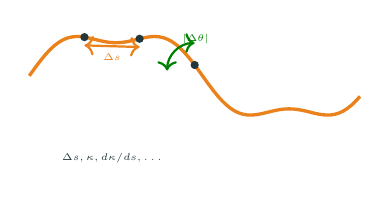
\begin{tikzpicture}[scale=0.7, transform shape]
  \draw[mLightBrown, very thick] plot[domain=0:6, samples=80]
        ({\x}, {0.8*sin(deg(\x)) + 0.2*sin(deg(3*\x))});
  \node[circle, fill=mDarkTeal, inner sep=1.5pt] at (1.0, {0.8*sin(deg(1.0)) + 0.2*sin(deg(3.0))}) {};
  \node[circle, fill=mDarkTeal, inner sep=1.5pt] at (2.0, {0.8*sin(deg(2.0)) + 0.2*sin(deg(6.0))}) {};
  \node[circle, fill=mDarkTeal, inner sep=1.5pt] at (3.0, {0.8*sin(deg(3.0)) + 0.2*sin(deg(9.0))}) {};
  \node[font=\tiny, mDarkTeal] at (1.5, -1.5) {$\Delta s, \kappa, d\kappa/ds, \ldots$};
  \draw[<->, accent, thick] (1.0, {0.8*sin(deg(1.0)) + 0.2*sin(deg(3.0)) - 0.15})
      -- (2.0, {0.8*sin(deg(2.0)) + 0.2*sin(deg(6.0)) - 0.15})
      node[midway, below, font=\tiny\itshape, accent] {$\Delta s$};
  \draw[<->, success, thick] (3.0, {0.8*sin(deg(3.0)) + 0.2*sin(deg(9.0)) + 0.4})
      arc (90:180:0.5) node[midway, above right, font=\tiny\itshape, success] {$|\Delta\theta|$};
\end{tikzpicture}\\[0.3em]
\scriptsize\textit{Các đại lượng nội tại được tính trên từng cặp điểm liền kề.}\\[0.6em]
\textcolor{accent}{$\Rightarrow$ Pipeline 7 kênh có \textbf{0} kênh phụ thuộc khung quy chiếu.}
\end{columns}
\end{frame}

% --- Step 2: Backbone architecture ---
\begin{frame}{Bước 2: Kiến trúc SE2RoadNet}
\begin{center}
\begin{tikzpicture}[
    box/.style={draw=mDarkTeal, thick, rounded corners, fill=tealtint!40,
                minimum width=3.2cm, minimum height=0.7cm, align=center, font=\scriptsize},
    arr/.style={-Stealth, thick, mLightBrown}
]
  \node[box] (proj) {Linear $7 \to 192$ + LayerNorm + GELU};
  \node[box, below=0.35cm of proj] (cls) {Concat token [CLS]};
  \node[box, below=0.35cm of cls, fill=mLightBrown!18, minimum width=3.6cm] (blk1) {InvariantBlock $\times 6$};
  \node[box, below=0.35cm of blk1] (pool) {Pool theo [CLS]};
  \node[box, below=0.35cm of pool, fill=success!18] (head) {Head: LN $\to 64 \to 1$};

  \draw[arr] (proj) -- (cls);
  \draw[arr] (cls) -- (blk1);
  \draw[arr] (blk1) -- (pool);
  \draw[arr] (pool) -- (head);

  \node[right=0.6cm of proj, font=\tiny, mDarkTeal, text width=4.8cm]
        {Mỗi điểm trên đường $\Rightarrow$ một token 192 chiều.};
  \node[right=0.6cm of blk1, font=\tiny, mDarkTeal, text width=4.8cm]
        {\textbf{Mỗi block} = MHA (8 heads) + FFN (512) + LayerNorm.\\
         Attention có \textbf{relative arclength bias}.};
  \node[right=0.6cm of head, font=\tiny, mDarkTeal, text width=4.8cm]
        {Output: 1 logit -- xác suất FAIL.\\\textbf{Tổng: 2.11 M tham số.}};
\end{tikzpicture}
\end{center}
\end{frame}

% --- Step 3: Equivariant attention ---
\begin{frame}{Bước 3: Attention với bias hiệu số $\Delta s$}
\begin{columns}[T]
\column{0.50\textwidth}
\begin{block}{Vấn đề với attention chuẩn}
\scriptsize
Position encoding chuẩn (sin/cos của index $i$) khoá mô hình vào \textbf{vị trí tuyệt đối} của token trong chuỗi. Khi đường được xoay/cắt khác, index $i$ tương ứng với arclength khác $\Rightarrow$ vỡ tính bất biến.
\end{block}

\begin{block}{Giải pháp: relative-arclength RFF bias}
\scriptsize
Thay vì PE tuyệt đối, ta thêm bias \emph{vào attention matrix} chỉ phụ thuộc \textbf{hiệu số} $\Delta s_{ij} = s_i - s_j$ (vốn là bất biến tái tham số hoá):
\vspace{-0.2em}
\[
\mathrm{bias}_{ij} \;=\; \mathrm{MLP}\bigl(\sin(\Delta s_{ij} \cdot \omega)\bigr) \in \mathbb{R}^{n_{\text{head}}}
\]
với $\omega \in \mathbb{R}^{32}$ là tần số Fourier ngẫu nhiên (RFF) cố định.
\end{block}

\begin{alertblock}{Chi phí}
\scriptsize
$\mathcal{O}(B \cdot L^2 \cdot 32)$ mỗi block -- chính là điểm tốn kém nhất (24 phút train). Cải tiến tương lai: RoPE-1D trên $s_{\text{norm}}$.
\end{alertblock}

\column{0.48\textwidth}
\centering
\safeincludegraphics[width=\linewidth, keepaspectratio]{fig_attention_relative.png}{Gemini: attention voi relative arclength bias}\\[0.3em]
\scriptsize\textit{Bias attention chỉ phụ thuộc $\Delta s_{ij}$, không bao giờ $i, j$ riêng lẻ.}
\end{columns}
\end{frame}

% --- Step 4: Training ---
\begin{frame}{Bước 4: Huấn luyện}
\begin{columns}[T]
\column{0.52\textwidth}
\begin{block}{Focal Loss -- tại sao không dùng BCE thuần?}
\scriptsize
\[
\mathcal{L} \;=\; -\,\alpha (1 - \hat{p}_t)^\gamma \log \hat{p}_t, \qquad \gamma = 1.5.
\]
\textbf{Vấn đề}: FAIL chỉ chiếm $\sim$30--40\% tập train. Với BCE thuần, model nhanh chóng học cách \emph{đoán PASS cho tất cả} $\Rightarrow$ loss thấp nhưng ranking vô nghĩa.\\[2pt]
\textbf{Cơ chế}: hệ số $(1-\hat{p}_t)^\gamma$ \emph{down-weight} các ví dụ dễ (PASS rõ ràng, $\hat{p}_t \approx 0$) và \emph{up-weight} các ví dụ khó (FAIL bị phân loại sai, $\hat{p}_t$ cao).\\[2pt]
\textbf{Chọn $\gamma = 1.5$}: $\gamma = 0$ suy biến về BCE; $\gamma$ quá cao chỉ train trên outlier cực đoan, mất ổn định. $\gamma = 1.5$ là điểm cân bằng thực nghiệm.
\end{block}

\column{0.44\textwidth}
\begin{block}{Cấu hình}
\scriptsize
\begin{tabular}{l l}
Optimizer       & AdamW (wd $=$ 1e-3)            \\
Learning rate   & 5e-4 cosine + warmup 5         \\
Batch size      & 384                            \\
Epochs          & 80 (SWA từ ep 56)              \\
Mixed precision & bf16                           \\
Sampler         & WeightedRandom (pos-weight)    \\
Wall-clock      & 24.2 phút (Kaggle Blackwell)   \\
Tham số         & \textbf{2.11 M}                \\
\end{tabular}
\end{block}

\begin{exampleblock}{Một chi tiết quan trọng}
\scriptsize
Eval chia chunk (\texttt{predict\_chunked}, batch 128) để tránh OOM khi tính bias $\Delta s$ trên toàn validation.
\end{exampleblock}
\end{columns}
\end{frame}

% --- Pipeline summary ---
\begin{frame}{Tổng kết bước phương pháp: Pipeline hoàn chỉnh}
\begin{center}
\safeincludegraphics[width=0.94\textwidth, keepaspectratio]{fig_pipeline_blocks.png}{Gemini: pipeline tong the SE2RoadNet}
\end{center}
\vspace{0.2em}
\begin{exampleblock}{Đọc lại pipeline theo chiều top-down}
\scriptsize
\textbf{Đầu vào} $(N, 2) \to$ \textbf{7 kênh bất biến} $\to$ \textbf{6 InvariantBlock} với MHA + relative-$\Delta s$ bias $\to$ \textbf{Focal BCE loss} ($\gamma{=}1.5$) $\to$ \textbf{SWA averaging} $\to$ \textbf{$\hat{p}_{\text{FAIL}}$}.
\end{exampleblock}
\end{frame}

% ============================================================
% PART IV -- EVALUATION
% ============================================================
\section{Đánh giá}

% --- APFD ---
\begin{frame}{Chỉ số đánh giá: APFD}
\begin{columns}[T]
\column{0.50\textwidth}
\begin{block}{Average Percentage of Faults Detected}
\small
Với hoán vị $\pi$ trên $n$ test (trong đó $m$ là FAIL), gọi $TF_i$ là vị trí của fault thứ $i$ trong $\pi$:
\[
\mathrm{APFD}(\pi) \;=\; 1 - \frac{\sum_{i=1}^{m} TF_i}{n \cdot m} + \frac{1}{2n}.
\]
\textbf{Khoảng giá trị}: $\mathrm{APFD} \in [0, 1]$, càng cao càng tốt.\\[3pt]
\textbf{Random}: $\approx 0.5$. \quad \textbf{Perfect}: $\approx 1.0$.
\end{block}

\column{0.48\textwidth}
\centering
\safeincludegraphics[width=\linewidth, keepaspectratio]{sensodat_apfd_curve.png}{Kaggle: APFD curve -- perfect vs SE2 vs random}\\[0.3em]
\scriptsize\textit{Đường cong APFD: ranking tốt $\Rightarrow$ phát hiện lỗi sớm $\Rightarrow$ đường cong tăng dốc đứng từ đầu.}
\end{columns}
\end{frame}

% --- Eval protocol ---
\begin{frame}{Giao thức đánh giá}
\begin{columns}[T]
\column{0.46\textwidth}
\begin{block}{Tập đánh giá}
\small
\begin{itemize}
    \item \textbf{Competition split} -- out-of-distribution (956 tests).
\end{itemize}
\end{block}

\begin{block}{Multi-trial APFD}
\small
\begin{itemize}
    \item \textbf{30 trials}.
    \item Mỗi trial: lấy ngẫu nhiên 287/956 tests, tính APFD, báo cáo $\overline{\mathrm{APFD}} \pm \sigma$.
    \item Loại bỏ ``may rủi'' do thứ tự cố định.
\end{itemize}
\end{block}

\begin{block}{Rotation probe}
\small
Xoay \emph{toàn bộ} Competition split bằng 6 góc $\{0, +30, +60, +90, +180, -45\}^\circ$ rồi đánh giá lại. Đo $\Delta = \max - \min$ APFD.
\end{block}

\column{0.50\textwidth}
\centering
\safeincludegraphics[width=\linewidth, keepaspectratio]{fig_eval_protocol.png}{Gemini: 3-panel protocol -- single / multi-trial / rotation}\\[0.3em]
\scriptsize\textit{Giao thức gồm 3 phần: single-pass / multi-trial / rotation probe.}
\end{columns}
\end{frame}

% --- HEADLINE rotation invariance ---
\begin{frame}{Kết quả: Bất biến phép xoay $\Delta = 0$}
\vspace{0.4em}
\begin{center}
\small
\begin{tabular}{l c c c c c c c}
\toprule
\textbf{Phép xoay} & $0^\circ$ & $+30^\circ$ & $+60^\circ$ & $+90^\circ$ & $+180^\circ$ & $-45^\circ$ & $\Delta$ \\
\midrule
ITEP4SDC (sota ICST 2025) & 0.7810 & 0.7240 & 0.7518 & 0.7396 & 0.7334 & 0.7627 & \alert{0.0570} \\
\textbf{SE2RoadNet}        & \textbf{0.8047} & \textbf{0.8047} & \textbf{0.8047} & \textbf{0.8047} & \textbf{0.8047} & \textbf{0.8047}
                           & \cellcolor{success!25}\textbf{0.0000} \\
\bottomrule
\end{tabular}
\end{center}

\vspace{0.8em}
\begin{exampleblock}{Đây không phải ``trong sai số'' -- mà là \emph{bit-identical}}
\small
6 lần đánh giá, 6 góc xoay khác nhau, APFD \textbf{bằng nhau đến đúng từng bit float}. Không phải $\sim 10^{-3}$, mà $= 0$ tuyệt đối. Lý do: pipeline 7 kênh trả về vector \emph{pixel-identical} sau khi xoay $\Rightarrow$ forward pass deterministic $\Rightarrow$ logit y nguyên.
\end{exampleblock}

\vspace{0.4em}
\centering\textcolor{accent}{$\Rightarrow$ \textbf{Lý thuyết được xác minh bằng thực nghiệm}, không cần nói ``xấp xỉ''.}
\end{frame}

% ============================================================
% PART V -- LEADERBOARD
% ============================================================
\section{Leaderboard}

\begin{frame}{So sánh với 8 baselines}
\small
\begin{center}
\begin{tabular}{l l c c c}
\toprule
\textbf{Phương pháp} & \textbf{Mô hình/Hệ thống} & \textbf{AUC} & \textbf{APFD} & \textbf{Bất biến SE(2)?} \\
\midrule
Random              & Cơ bản                 & --     & 0.493 & không \\
LLM zero-shot       & Mô hình ngôn ngữ lớn   & --     & 0.487 & không \\
GNN                 & Đồ thị đường           & --     & 0.533 & không \\
ResNet-50 visual    & CNN ảnh đường          & --     & 0.572 & không \\
SO-SDC-Prioritizer  & GA đơn mục tiêu        & --     & 0.765 & không \\
ITEP4SDC            & MLP, 3 đặc trưng       & --     & 0.781 & không \\
Greedy-diversity    & Heuristic đa dạng      & --     & 0.795 & không \\
RoadFury            & Transformer + SWA      & 0.917  & 0.804 & không \\
\midrule
\rowcolor{success!15}
\textbf{SE2RoadNet} & \textbf{Group-equivariant} & \textbf{0.934} & \textbf{0.804}
        & \cellcolor{success!25}\textbf{$\Delta = 0$ EXACT} \\
\bottomrule
\end{tabular}
\end{center}

\vspace{0.6em}
\begin{exampleblock}{Đọc bảng}
\small
SE2RoadNet \textbf{ngang APFD} với baseline tốt nhất, nhưng \textbf{tăng AUC} (+0.017) và \textbf{thêm guarantee lý thuyết} mà không phương pháp nào trên có. Đây là một \emph{``strict improvement''} theo nghĩa Pareto.
\end{exampleblock}
\end{frame}

% ============================================================
% PART VI -- Q&A
% ============================================================
\section{Q\&A}

\begin{frame}
\centering
\vspace{0.8em}
{\Huge Cảm ơn thầy đã lắng nghe!}\\[0.7em]
{\Large \textcolor{accent}{Q\&A}}

\vspace{1.6em}
{\normalsize \textbf{Test Prioritization for Self-Driving Cars}}\\[0.3em]
{\scriptsize Trần Chí Nguyên \quad $\cdot$ \quad Huỳnh Trung Kiệt \quad $\cdot$ \quad Đào Sỹ Duy Minh}\\[0.2em]
{\scriptsize University of Science, VNU-HCM \quad $\cdot$ \quad ICST 2026}
\end{frame}

\end{document}
